\documentclass{beamer}
\usetheme{Madrid}

\setbeamertemplate{title page}{
  \vbox{}
  \vfill
  \begingroup
    \centering
    \usebeamertemplate{title}
    \usebeamertemplate{author}
    \vskip1.5em
    \usebeamertemplate{date}
    \vskip1.5em
    \usebeamertemplate{institute}
    \usebeamertemplate{titlegraphic}
  \endgroup
  \vfill
}


\title{Physics Research Showcase}
\subtitle{Numerical solutions to the DGLAP equations}
\author{Casey Hampson}
\addtobeamertemplate{author}{}{Supervisor: Marco Guzzi\par}
\date{18 April, 2025}
\institute[]{NSF Grant: PHY-2412071}
\titlegraphic{
\includegraphics[width=0.1\textwidth]{./gfx/nsf-logo.png}}



\usepackage{amsmath}
\usepackage{amssymb}
\usepackage{siunitx}
\usepackage{mathtools}
\usepackage{esdiff}
\usepackage{esint}
\usepackage{bm}
\usepackage{tikz-feynman}
\usepackage{wrapfig}

\newcommand{\dd}{\mathrm{d}}
\newcommand{\vv}[1]{\mathbf{\bm{#1}}}


\begin{document}
\frame{\titlepage}



\begin{frame}
  \frametitle{Introduction}

  \begin{itemize}
  \item High-energy physicists are tasked with determining the behavior of the universe on the smallest possible scales.
  \item The particle accelerator located at CERN in Geneva, Switzerland provides us with a unique opportunity to answer some of our most important questions about physics.
  \item Some of these include:
    \begin{itemize}
    \item Dark matter and dark energy
    \item Properties of the Higgs boson, discovered at CERN in 2012
    \item The origin of mass, the spin of the proton
    \item New particles and interactions
    \end{itemize}
  \end{itemize}

  \begin{figure}
    \centering
    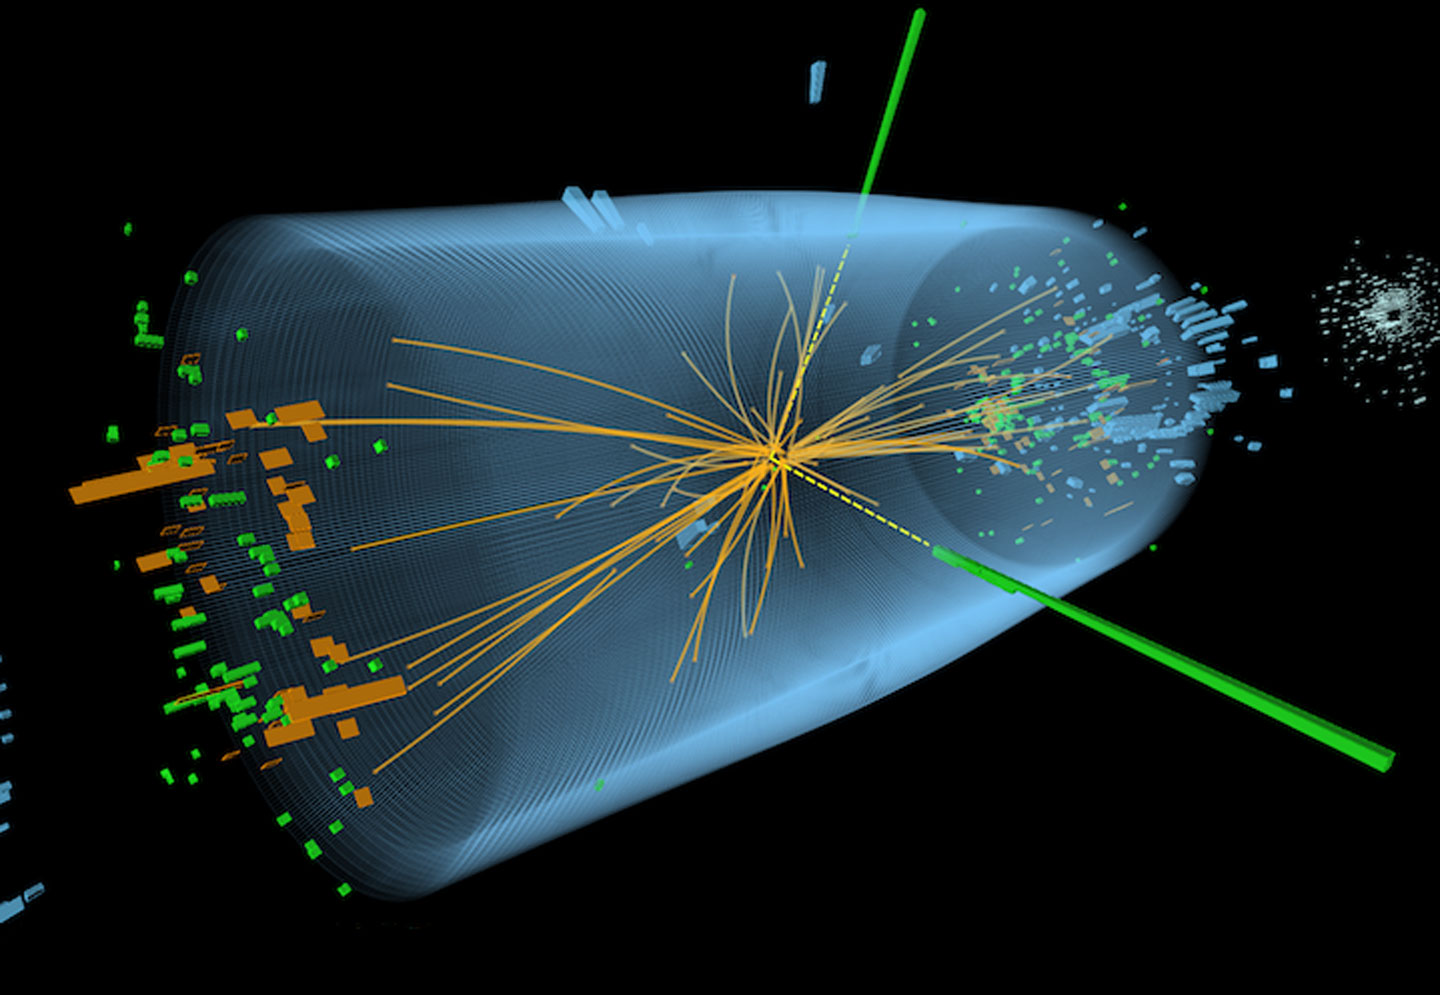
\includegraphics[width=0.35\linewidth]{./gfx/lhc.jpg}
  \end{figure}
  
\end{frame}


\begin{frame}
  \frametitle{The LHC at CERN in Geneva, Switzerland}

  \begin{itemize}
  \item The LHC at CERN collides protons at nearly the speed of light around a 16.8 mile ring.
  \item At such high energies, the proton's structure breaks down, resulting in a multitude of particles in the final state.
  \end{itemize}

  \begin{figure}
    \centering
    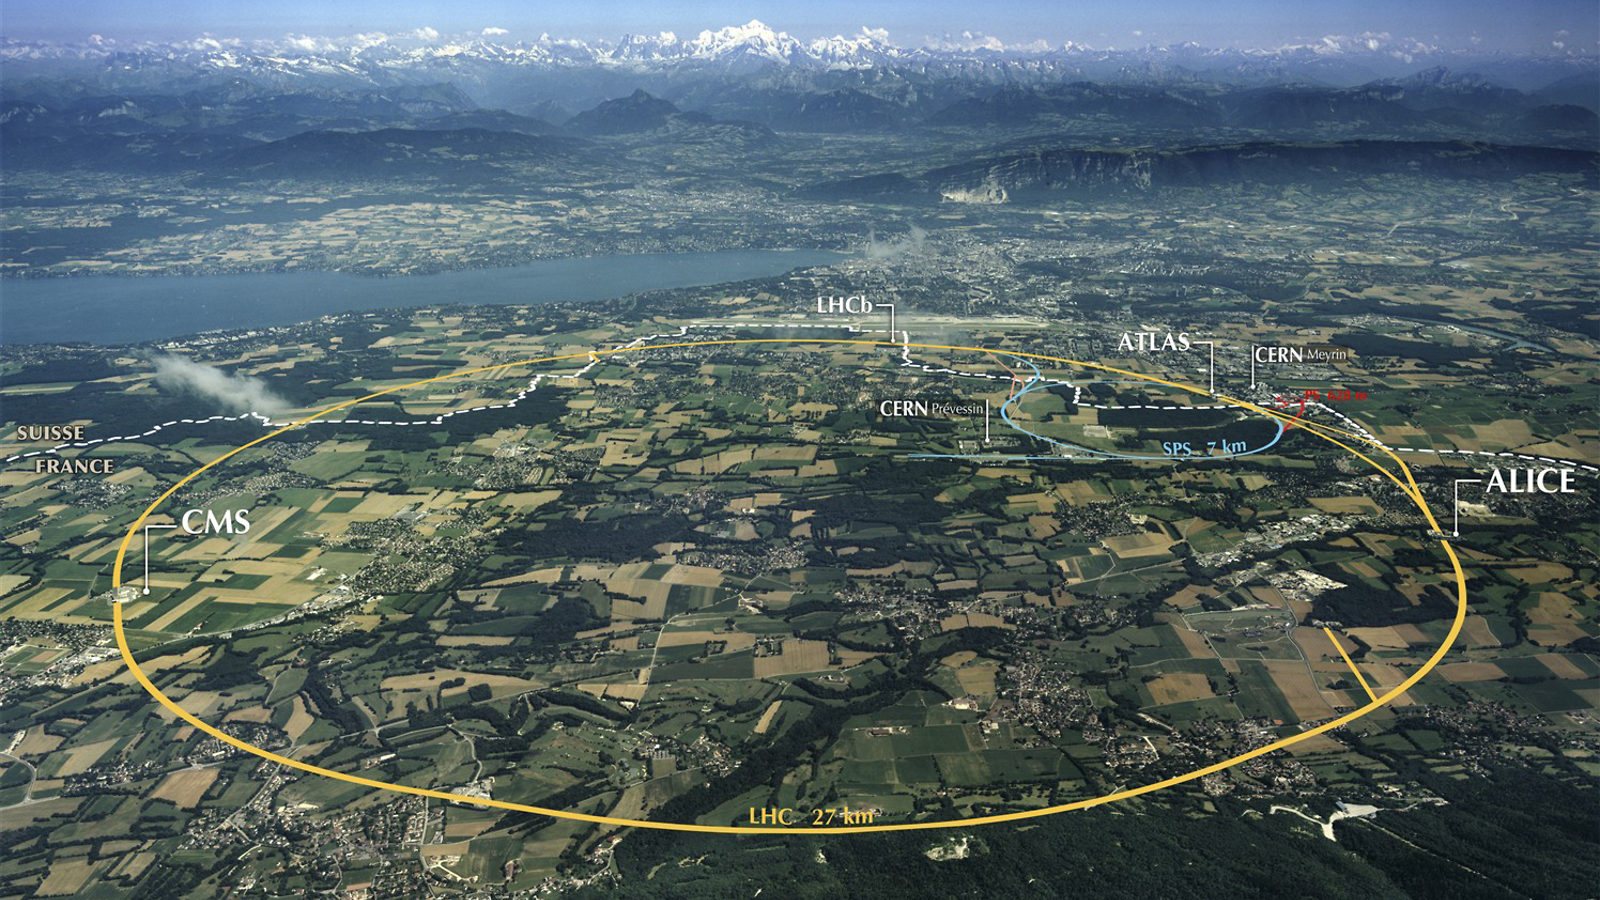
\includegraphics[width=0.7\linewidth]{./gfx/lhc-map.jpg}
  \end{figure}
\end{frame}


\begin{frame}
  \frametitle{Introduction}

  \begin{itemize}
  \item The LHC and future Electron-Ion-Collider (EIC) to be built at Brookhaven National Laboratory in the US, provide us with measurements at unparalleled precision.
  \item It allows us to set stringent tests on the Standard Model
  \item It also allows us to search for signatures of new physics, such as new particles or interactions
  \end{itemize}


  \begin{figure}
    \centering
    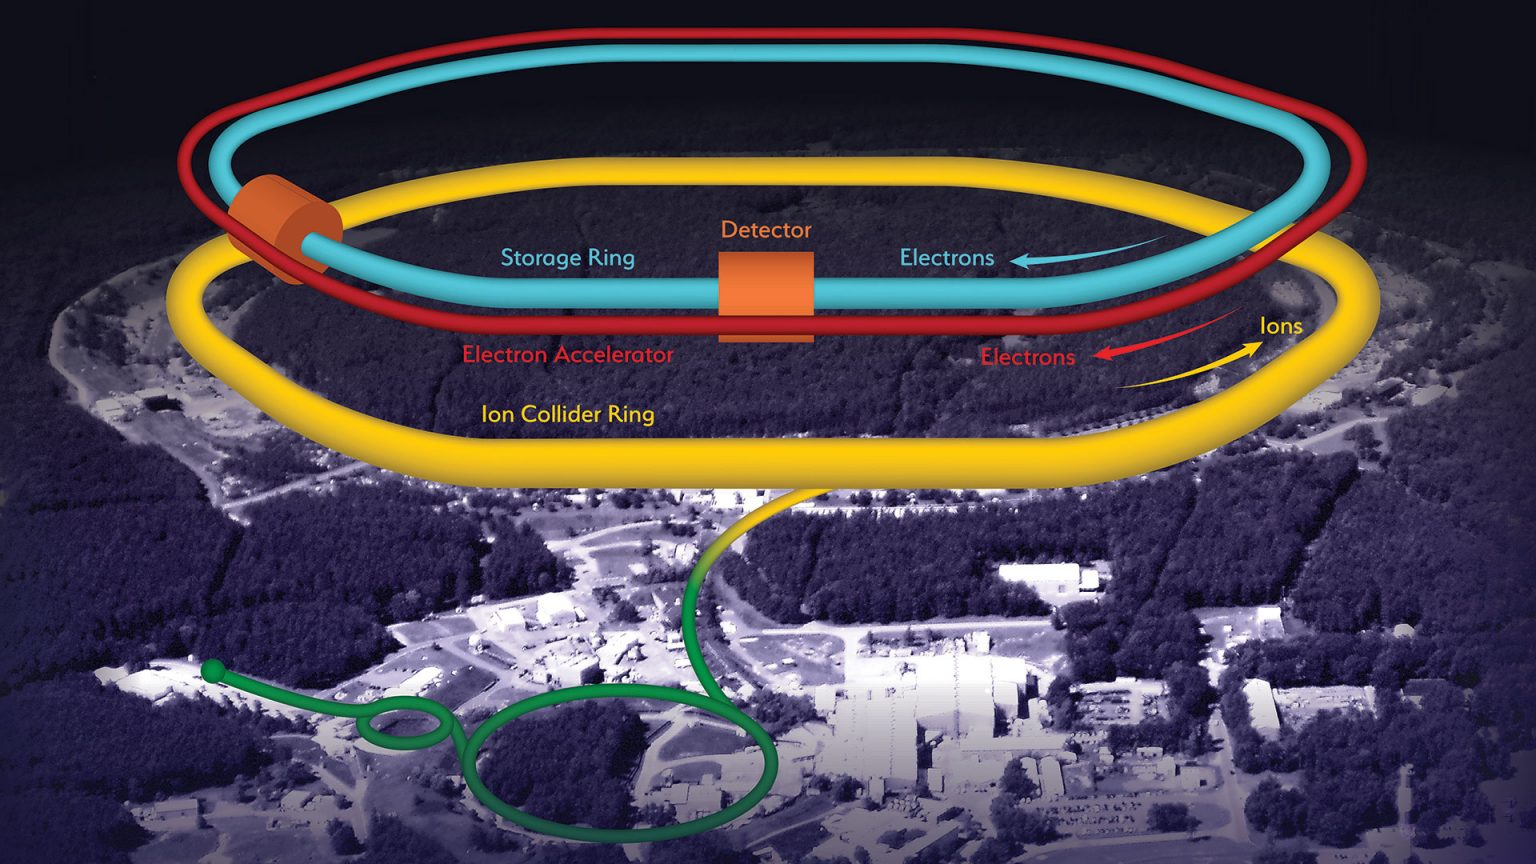
\includegraphics[width=0.44\linewidth]{./gfx/eic.jpg}
    \caption{Schematic of the EIC.}
  \end{figure}
\end{frame}


\begin{frame}
  \frametitle{The Standard Model of Particle Physics}


  \begin{figure}
    \centering
    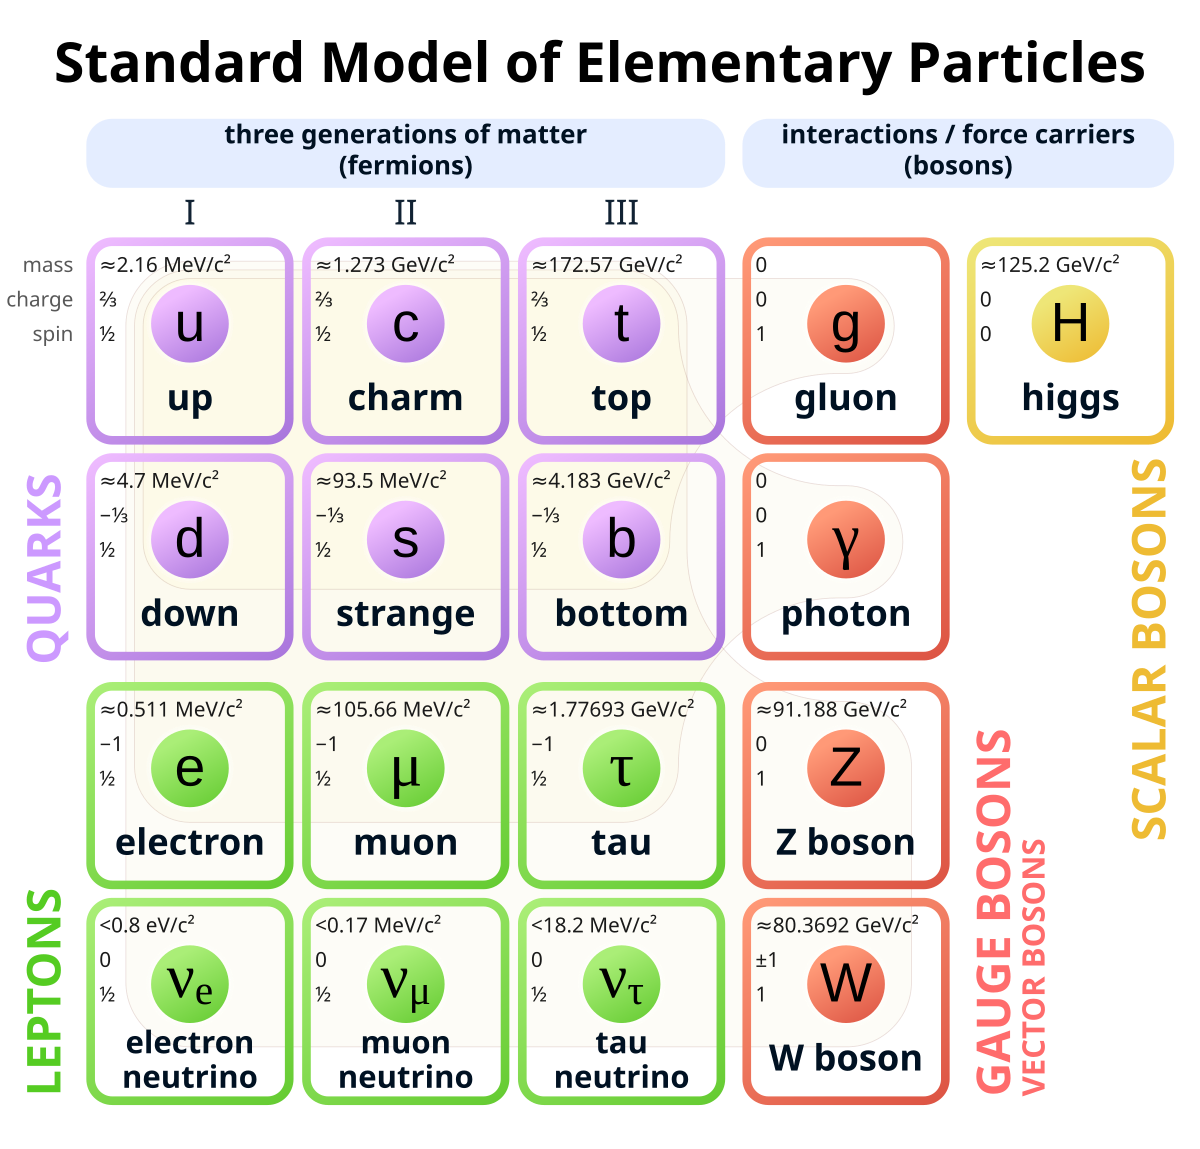
\includegraphics[width=0.4\linewidth]{./gfx/standard-model.png}
  \end{figure}

  \begin{itemize}
  \item The Standard Model is the work of decades of research and represents our best theory of the universe.
  \item The Higgs boson, was the most recently added particle, having been discovered in 2012 at the LHC
  \end{itemize}

\end{frame}



\begin{frame}
  \frametitle{Photos from Summer 2024 REU at CERN}

  \begin{figure}
    \centering
    \includegraphics<1>[width=0.6\linewidth]{./gfx/cern/1.jpg}
    \includegraphics<1>[width=0.6\linewidth]{./gfx/cern/2.jpg}
    \includegraphics<2>[width=0.6\linewidth]{./gfx/cern/3.jpg}
    \includegraphics<2>[width=0.6\linewidth]{./gfx/cern/4.jpg}
  \end{figure}
  
\end{frame}


\begin{frame}
  \frametitle{Cross Sections}

  \begin{itemize}
  \item What is measured in these colliders is the \textbf{cross section}, which roughly corresponds to probabilities for interactions to occur.
  \item As theorists, we are also able to calculate these quantities and compare them to what we observe in the experiment.
  \end{itemize}

  \begin{equation}
    \frac{N_{\mathrm{ev}}}{\mathrm{sec}} = L \cdot \sigma,
  \end{equation}

  \begin{itemize}
  \item $L$ is the \textbf{luminosity}, which describes the number of collisions that can be produced per $\mathrm{cm}^2$ per second.
  \item $\sigma$ is the cross section.
  \end{itemize}
\end{frame}


\begin{frame}
  \frametitle{Cross Sections}

  \begin{itemize}
  \item The theoretical calculation of a cross section can be split up like so:
  \end{itemize}

  \begin{equation}
    \sigma = \sum_{\text{partons}=i,j} f_i \otimes f_j \otimes \hat{\sigma}_{ij}.
  \end{equation}

  \begin{itemize}
  \item The functions $f_i$ and $f_j$ are \textbf{parton distribution functions} (PDFs) of the proton, and give a probability for finding a parton (the proton's constituent quarks and gluons) with a certain longitudinal momentum fraction at a particular energy scale.
  \item $\hat{\sigma}_{ij}$ is the \textit{partonic} cross section containing information purely about the interaction between the $i$ and $j$ partons.
  \end{itemize}
\end{frame}


\begin{frame}
  \frametitle{What happens in collisions?}

  \begin{itemize}
  \item At such high speeds, because special relativity, the protons get length contracted and appear as disks
  \item The inner constituents are spread throughout and collide with those of the other length-contracted proton.
  \end{itemize}

  \begin{figure}
    \centering
    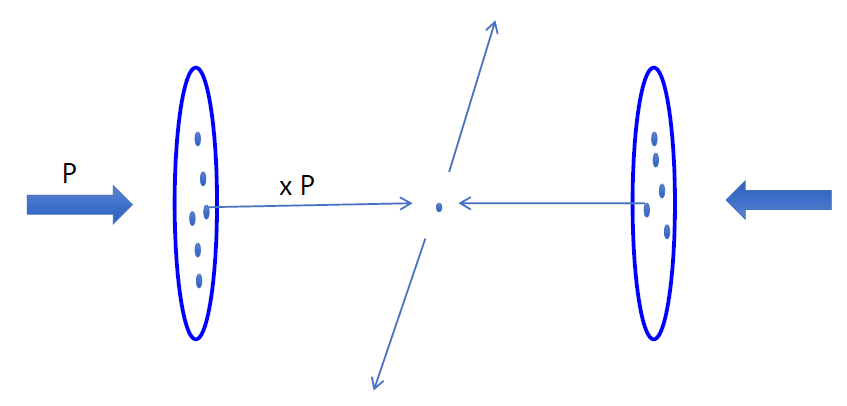
\includegraphics[width=0.6\linewidth]{./gfx/colliding-protons.png}
  \end{figure}

  \begin{itemize}
  \item The PDFs encode the longitudinal momentum fractions that the partons have when they collide.
  \end{itemize}
\end{frame}



\begin{frame}
\frametitle{Parton Distribution Functions}

\begin{itemize}
\item PDFs are particularly challenging because these are quantities that we cannot compute from first principles, they must be determined from experiment.
\item We can, however, given a distribution at some initial energy scale, predict how they evolve with energy and determine the distributions at another scale.
\item This energy dependence is encoded in the DGLAP equations.
\end{itemize}

\begin{figure}
  \centering
  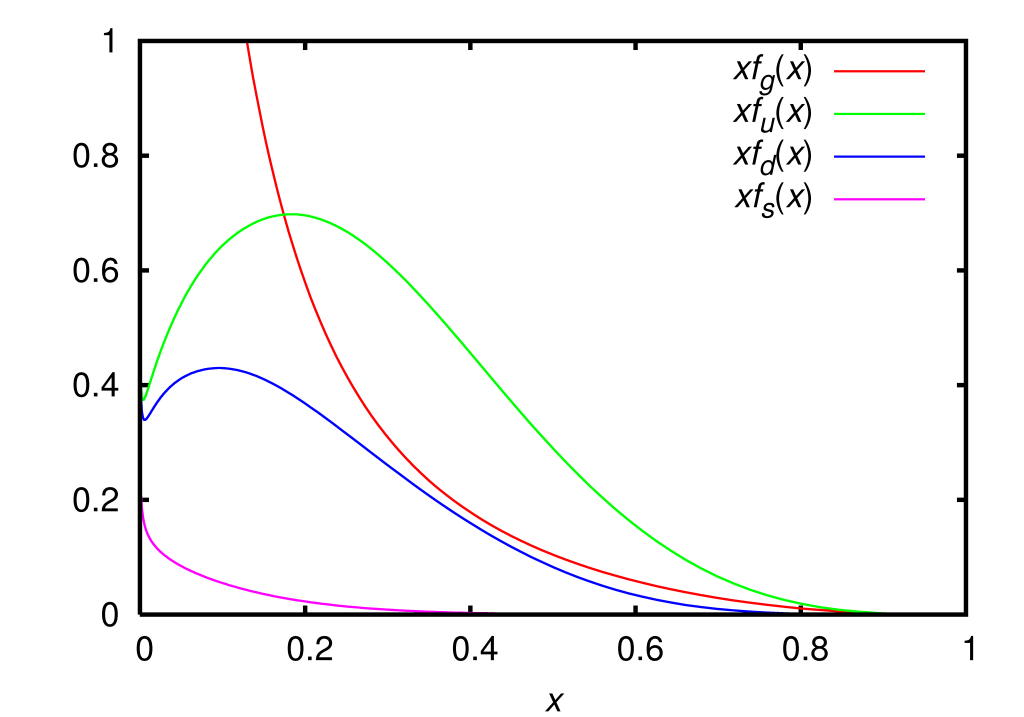
\includegraphics[width=0.4\linewidth]{./gfx/pdfs.png}
\end{figure}

\end{frame}


\begin{frame}
  \frametitle{DGLAP Evolution Equations}

  \begin{itemize}
  \item The DGLAP equations describe how the PDFs evolve with energy.
  \item They are a set of integro-differential equations that go like:
  \end{itemize}

  \begin{equation}
    \frac{\partial}{\partial \ln Q^2} = P(x, \alpha_s(Q^2)) \otimes f(x, Q^2),
  \end{equation}

  where $f$ is the PDF, $\alpha_s$ is the strong coupling constant, and $P$ is the \textit{splitting function}, which roughly corresponds to probabilities for quarks to emit gluons and vice versa. The $\otimes$ corresponds to a convolution, defined like so:

  \begin{equation}
    [a \otimes b](x) = \int_x^1 \frac{\dd y}{y} a\left( \frac{x}{y} \right) b(y) = \int_x^1 \frac{\dd y}{y} a(y) b\left( \frac{x}{y} \right).
  \end{equation}

\end{frame}


% for this slide, remove most of the stuff and simply mention other methods
% which have some pros and cons, but we want to remain in x since that's real life space
% and we keep the analytical/mathematical structure
\begin{frame}
  \frametitle{Solutions to the DGLAP Equations}

  \begin{itemize}
  \item Solutions are particularly challenging due to the convolution appearing on the R.H.S.
  \item There are many mathematical tricks to employ, such as transforming to different spaces such as Laplace or Mellin transforms.
  \item In the latter case, it turns the convolution into a simple algebraic product, but there is additional time spent on transforming to and from Mellin space.
  \end{itemize}

  \begin{itemize}
  \item We work directly in $x$-space ($x$ being the original longitudinal momentum fraction) because this keeps the mathematical/analytical structure of the equations intact.
  \item It also avoids having to made additional transforms to and from some other space.
  \end{itemize}
\end{frame}
  


\begin{frame}
  \frametitle{The Non-singlet Case}

  \begin{itemize}
  \item There are two classes of solutions called ``singlet'' and ``non-singlet.'' The singlet case involves matrices, and the non-singlet involves scalars. The non-singlet case is therefore much more simple.
  \item For this case at Leading Order (LO), one particular ansatz that evolves the PDF $f$ from an initial scale $Q_0^2$ to a final scale $Q^2$ is given by:
  \end{itemize}

  \begin{equation}
    f(x, Q^2) = \sum_{n=0}^{\infty} \frac{A_n(x)}{n!} \ln^n\left( \frac{a_s(Q^2)}{a_s(Q_0^2)} \right),
  \end{equation}

  \begin{itemize}
  \item The $A_n(x)$s satisfy a recursion relation:
  \end{itemize}

  \begin{equation}
    A_{n+1}(x) = - \frac{2}{\beta_0}[P^{(0)} \otimes A_n] (x).
  \end{equation}
\end{frame}


\begin{frame}
  \frametitle{The Non-singlet Case}

  \begin{itemize}
  \item At $NLO$ the ansatz looks roughly the same, but of course with higher order terms 
  \end{itemize}

  \begin{equation}
    f(x, Q^2) = \sum_{n=0}^{\infty}\sum_{s=0}^n \frac{B_n^s(x)}{n!(s-n)!} \ln^n \left( \frac{\alpha_s}{\alpha_0} \right) \ln^{s-n}\left( \frac{4\pi\beta_0 + \alpha_s\beta_1}{4\pi\beta_0 + \alpha_0\beta_1} \right).
  \end{equation}

  \begin{itemize}
  \item The $B_s^n(x)$s will follow more advaned recursion relations as well, i.e. all the $n\neq0$ coefficients first.
  \item Generalizing this to $N^3LO$ is one of our main goals.
  \end{itemize}
\end{frame}


\begin{frame}
  \frametitle{Singlet Ansatz}

  \begin{itemize}
  \item For the singlet case, which are matrices, we consider the following ansatz:
  \end{itemize}

  \begin{equation}
    \vv{f}(x, Q^2) = \left[ 1 + \sum_{k=0}^{\kappa} \alpha_s^k \vv{U}_k \right] \otimes \vv{L} \otimes \left[ 1 + \sum_{k=0}^{\kappa} \alpha_0^k \vv{U}_k \right]^{-1} \otimes \vv{f}(x, Q_0^2).
  \end{equation}

  \begin{itemize}
  \item Here, the $\vv{U}_k$ matrices contain information related to the splitting function which we would keep to only $N^3LO$, but the index $\kappa$ is called a \textit{truncation index}, which in principle we would take to infinity, but practically must keep finite.
  \item In $x$-space, the regular products of these matrices would turn into convolutions. This is currently being tested.
  \end{itemize}
\end{frame}


\begin{frame}
  \frametitle{Current Progress}

  \begin{itemize}
  \item We are currently working with the literature to begin including the most up-to-date version of the $N^3LO$ splitting functions into our code.
  \item The previous \textsc{Candia} code was written in C, but has since been upgraded to C++ with a few minor optimizations. Once the new singlet ansatz and aforementioned splitting function corrections are added we will release the code and call it \textsc{Candia-v2} along with a publication. Time will be spent on improving the algorithm and making further optimizations.
  \item On the next slide are example outputs/plots for the current version of the program.
  \end{itemize}
\end{frame}


\begin{frame}
  \frametitle{Example Outputs: $u$ quark Distribution}

  \begin{figure}
    \centering
    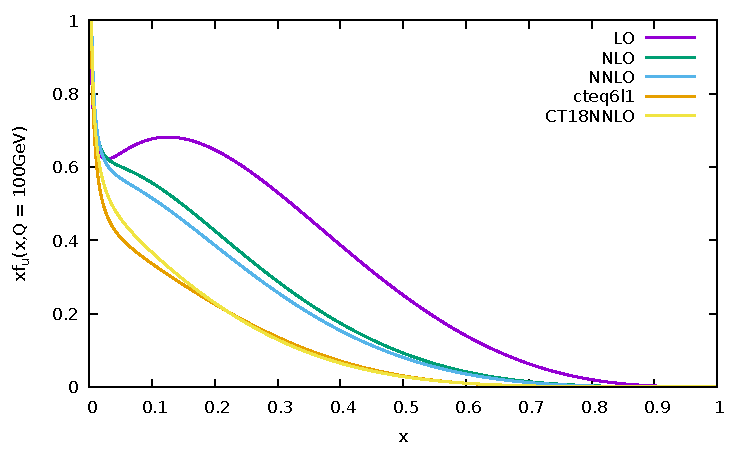
\includegraphics[width=0.75\linewidth]{./gfx/u.pdf}
  \end{figure}
\end{frame}



\begin{frame}
  \frametitle{Conclusions}

  \begin{itemize}
  \item A large portion of uncertainly in theoretical predictions and simulations for proton-proton collisions lies in these calculations of the PDFs
  \item We are working to generalize the previous algorithm in \textsc{Candia} to include the $N^3LO$ splitting functions and more sophisticated ansatzes to further increase precision.
  \item Additional work is being done on improving computational speed and efficiency, particularly in the area of convolutions.
  \item The results will be published to a peer-reviewed journal and the new computer code, dubbed \textsc{Candia-v2} will be made publically available.
  \end{itemize}
\end{frame}


\end{document}

%%% Local Variables:
%%% mode: LaTeX
%%% TeX-master: t
%%% End:
